\documentclass[lualatex,handout]{beamer}
\setbeamertemplate{footline}[frame number]
%\useoutertheme{infolines}
\usepackage{luatexja}
\usepackage{xspace}
\usepackage{amsmath,amssymb}
\usepackage{mathtools}

\usepackage{tikz}
\usepackage{pgfplots}

%\usepackage[haranoaji]{luatexja-preset}
\usepackage[deluxe,ipaex]{luatexja-preset}
\renewcommand{\kanjifamilydefault}{\gtdefault}
%\setmainjfont{HaranoAjiGothic-Regular}

\usepackage{unicode-math}
%\setmathfont{Fira Math}
\setmathfont{STIX Two Math}
\setmathrm{STIX Two Math}[StylisticSet=8]
%\setmathfont{STIX Two Math}[range={up,it,bb,bbit,scr,bfscr},StylisticSet=8]
%\setmathfont{XITS Math}
%\setmathrm{XITS Math}[StylisticSet=8]
%\setmathfont{XITS Math}[StylisticSet=8]

%\usefonttheme{professionalfonts}

\usepackage{luacolor}

%\newcommand{\emm}[1]{\textcolor{red}{#1}}
%\newcommand{\emm}[1]{\color{red}#1\color{black}}
\newcommand{\mycolor}[2]{%
  \begingroup
  \colorlet{currentcolor}{.}%
  \color{#1}#2%
  \color{currentcolor}%
  \endgroup
}
\newcommand{\emm}[1]{\mycolor{red}{#1}}
\newcommand{\expt}[1]{\mathbb{E}\left[#1\right]}
\newcommand{\var}[1]{\mathbb{V}\left[#1\right]}
\newcommand{\cov}[1]{\mathrm{Cov}\left[#1\right]}


\newcommand\bm[1]{{\mathbf{#1}}}

\theoremstyle{definition}

\title{確率・統計基礎: 確率論の初歩}
\author{森 立平}
\date{}



\begin{document}
\begin{frame}[plain]
\maketitle
\end{frame}


\begin{frame}{確率とは}
\begin{itemize}
\setlength{\itemsep}{2em}
\item 世の中のランダムな事象を数学的に記述したもの
\item 統計・機械学習の基礎となっている
\item 極限定理: 確率$p$で表が出るコインを$N$回投げた時に、表が出る回数$F$は
\vspace{1em}
\begin{itemize}
\setlength{\itemsep}{1em}
\item 大数の法則: $\frac{F}{N} \to p$
\item 大偏差原理: $\Pr\left(\left|\frac{F}{N} - p\right| > \epsilon\right) = \mathrm{e}^{-\beta N}$
\item 中心極限定理: $\frac{F-pN}{\sqrt{N}}\to$正規分布
\end{itemize}
\end{itemize}
\end{frame}

\begin{frame}{統計とは}
確率論は統計の基礎となる
\vspace{1em}
\begin{itemize}
\item クラスタリング: この患者は病気ですか?
\item a
\end{itemize}
\end{frame}

\begin{frame}{確率論の数学モデルとは?}
\begin{center}
\large 測度論!
\end{center}

\vspace{1em}
\begin{itemize}
\setlength{\itemsep}{2em}
\item 確率は面積($=$測度)のようなもの。
\item 数学的に\textbf{厳密}に様々な結果(大数の法則、大偏差原理、中心極限定理)が証明できる。
\item とても重要だが勉強するのは3年生以降(解析学要論Ⅱ、確率論)。
\item この授業では\emm{測度論には深入りせず、基礎的な部分はごまかしながら確率・統計の重要な理論について学ぶ}。
\end{itemize}
\end{frame}

\begin{frame}{標本空間と確率}
\begin{itemize}
\setlength{\itemsep}{1em}
\item $\Omega\colon$ 集合。これの部分集合に確率が与えられる
\item $P\colon 2^\Omega\to[0,1].$ 確率を与える関数
\end{itemize}
\begin{example}
\small
\begin{itemize}
\setlength{\itemsep}{.51em}
\item $\Omega=\{表,裏\}$.
\item $P(\emptyset)= 0,\, P(\{\mathrm{表}\})=P(\{\mathrm{裏}\})=\frac12,\,P(\{\mathrm{表},\mathrm{裏}\})=1$.
\end{itemize}

\vspace{1.0em}
\begin{itemize}
\setlength{\itemsep}{.51em}
\item $\Omega=\{1,2,3,4,5,6\}$.
\item $P(A) = \frac{|A|}6\quad\forall A\subseteq\Omega$.
\end{itemize}

\vspace{1.0em}
\begin{itemize}
\setlength{\itemsep}{.5em}
\item $\Omega=\{晴,雨,雪\}$.
\item $P(\emptyset)= 0,\, P(\{晴\})=0.7,\, P(\{雨\})=0.2,\,P(\{雪\})=0.1$,\\
$P(\{晴,雨\})=0.9,\, P(\{雨,雪\})=0.3,\, P(\{雪,晴\})=0.8$\\
$P(\{晴,雨,雪\})=1$.
\end{itemize}
\end{example}
\end{frame}

\begin{frame}{確率論の公理有限版}
\begin{itemize}
\item $\Omega\colon$ \emm{有限}集合(\emm{標本空間})
\item $P\colon 2^\Omega\to[0,1]$ (\emm{確率測度})
\end{itemize}
\vspace{1em}
確率の公理
\begin{enumerate}
\item $P(\Omega)=1$.
\item $\forall A, B\subseteq\Omega$, $A\cap B=\emptyset\implies P(A\cup B)=P(A)+P(B)$\\ (\emm{有限加法性}).
\end{enumerate}

\vspace{2em}
\begin{center}
$\Omega$を無限集合にしたい場合はどうする?
\end{center}
\end{frame}

\begin{frame}{確率論の公理可算版}
\begin{itemize}
\item $\Omega\colon$ 高々\emm{可算}集合(\emm{標本空間})
\item $P\colon 2^\Omega\to[0,1]$ (\emm{確率測度})
\end{itemize}
\vspace{1em}
確率の公理
\begin{enumerate}
\item $P(\Omega)=1$.
\item {\color{lightgray}$\forall A, B\subseteq\Omega$, $A\cap B=\emptyset\implies P(A\cup B)=P(A)+P(B)$\\ (有限加法性).}\\
\item[2'.] $\forall (A_n\subseteq\Omega)_{n=1,\dotsc}$, $\forall i\ne j,\, A_i\cap A_j=\emptyset\implies P\left(\bigcup_{n=1}^\infty A_n\right)=\sum_{n=1}^\infty P(A_n)$\\ (\emm{完全加法性, $\sigma$-加法性}).
\end{enumerate}

%\vspace{2em}
%\begin{center}
%$\Omega$を非可算無限集合にしたい場合はどうする?
%\end{center}
\end{frame}

\begin{frame}{なぜ有限加法性じゃ駄目なの?$\leftarrow$駄目じゃないけど$\dotsc$}
\begin{theorem}[確率測度の連続性]
$P$を\emm{完全加法}確率測度とする。
事象$A_1\subseteq A_2\subseteq \dotsb$について
\begin{align*}
P\left(\bigcup_{i=1}^\infty A_i\right) = \lim_{n\to\infty} P(A_n).
\end{align*}
\end{theorem}
\begin{proof}
$B_1\coloneq A_1$, $i\ge 2$について$B_i\coloneq A_i\setminus A_{i-1}$とおく。
このとき、$i\ne j$について $B_i\cap B_j=\emptyset$。また、$\bigcup_{i=1}^n B_i = \bigcup_{i=1}^nA_i = A_n$.
\begin{align*}
P\left(\bigcup_{i=1}^\infty A_i\right)&= P\left(\bigcup_{i=1}^\infty B_i\right) \emm{=}\sum_{i=1}^\infty P(B_i)\\
&=\lim_{n\to\infty} \sum_{i=1}^n P(B_i)
=\lim_{n\to\infty} P\left(\bigcup_{i=1}^n B_i\right)
=\lim_{n\to\infty} P(A_n).\qedhere
\end{align*}
\end{proof}
\end{frame}

\begin{frame}{実数上の測度}
\begin{itemize}
\item $\Omega=[0,1)$.
\item $P\colon 2^\Omega\to[0,1]$
\end{itemize}
ここで
\begin{align*}
P([a, b]) = b-a
\end{align*}
となるようにしたい。
すると$P([a, a+\epsilon])=\epsilon$なので$P(\{a\})\le\epsilon$である。
任意の$\epsilon>0$について成り立つので$P(\{a\})=0$である。

\vspace{1em}
任意の1点の確率は0だけど全体の確率は1になるようにする。

なので\emm{加法性は非可算には一般化しない}。

\end{frame}

\begin{frame}{確率論の公理最終版?}
これでよいのか?
\begin{itemize}
\item $\Omega\colon$ (\emm{非可算}でもよい)集合(\emm{標本空間})
\item $P\colon 2^\Omega\to[0,1]$ (\emm{確率測度})
\end{itemize}
\vspace{1em}
確率の公理
\begin{enumerate}
\item $P(\Omega)=1$.
\item {\color{lightgray}$\forall A, B\subseteq\Omega$, $A\cap B=\emptyset\implies P(A\cup B)=P(A)+P(B)$\\ (有限加法性).}\\
\item[2'.] $\forall (A_n\subseteq\Omega)_{n=1,\dotsc}$, $\forall i\ne j,\, A_i\cap A_j=\emptyset\implies P\left(\bigcup_{n=1}^\infty A_n\right)=\sum_{n=1}^\infty P(A_n)$\\ (\emm{完全加法性, $\sigma$-加法性}).
\end{enumerate}

\vspace{2em}
\begin{center}
これで大丈夫?
\end{center}
%\vspace{2em}
%\begin{center}
%$\Omega$を非可算無限集合にしたい場合はどうする?
%\end{center}
\end{frame}

%\begin{frame}{$\mathcal{F} = 2^\Omega$にしたいです$\leftarrow$無理です(完全加法性+選択公理)}
\begin{frame}{ダメー(完全加法性+選択公理)}
\small
%確率空間$(\Omega,\mathcal{F},P)$が以下を満たすとする
\begin{itemize}
%\item $\Omega=[0,1)$, $\mathcal{F} = 2^\Omega$.
\item $\Omega=[0,1)$.
%\item $P([a,b]) = b-a$.
%\item $\forall c\in\Omega,\, A\in\mathcal{F},\, P(A+c) = P(A)$ where $A+c\coloneq\{a+c-\lfloor a+c\rfloor\mid a\in A\}$.
\item $\forall c\in\Omega,\, A\subseteq\Omega,\, P(A+c) = P(A)$ where $A+c\coloneq\{a+c-\lfloor a+c\rfloor\mid a\in A\}$.
\end{itemize}
\emm{選択公理を仮定するとそのような確率空間は存在しない}。

\vspace{1em}
$\Omega$の上の同値関係を
$x\sim y\stackrel{\mathrm{def}}{\iff} x-y \in\mathbb{Q}$と定義する。

\vspace{1em}
$\Omega$の上の同値類から一つずつ要素を選んで集合$V$を作る(選択公理)。
%
\begin{align*}
1 = P([0,1)) &= P\left(\bigcup_{x\in\mathbb{Q}} (V + x)\right)\\
&= \sum_{x\in\mathbb{Q}} P\left(V + x\right)\qquad\text{(完全加法性)}\\
&= \sum_{x\in\mathbb{Q}} P\left(V\right)
\end{align*}
\emm{同じ値を無限回足して1にはできない}。
\end{frame}


\begin{frame}{ちゃんとした確率論の公理}
\emm{確率空間} $(\Omega, \mathcal{F}, P)$

\vspace{.5em}
\begin{itemize}
\item $\Omega\colon$ 集合(\emm{標本空間})
\item $\mathcal{F}\subseteq 2^\Omega$ (\emm{事象の集合}、可測集合)
\item $P\colon\emm{\mathcal{F}}\to[0,1]$ (\emm{確率測度}、\emm{\small 確率は$\mathcal{F}$の要素にのみ定義される!})
\end{itemize}

\vspace{.5em}
可測集合の公理($\sigma$-加法族、完全加法族)
\begin{enumerate}
\item $\emptyset\in\mathcal{F}$.
\item $A\in\mathcal{F}\implies A^c\in\mathcal{F}$.
%\item $A,\,B\in\mathcal{F}\implies A\cup B\in\mathcal{F}$ (有限加法性).
\item[3'.] $(A_n\in\mathcal{F})_{n=1,\dotsc}\implies \bigcup_{n=1}^\infty A_n\in\mathcal{F}$ (完全加法性, $\sigma$-加法性).
\end{enumerate}

\vspace{.5em}
確率の公理
\begin{enumerate}
\item $P(\Omega)=1$.
%\item $\forall A, B\in\mathcal{F}$, $A\cap B=\emptyset\implies P(A\cup B)=P(A)+P(B)$\\ (有限加法性).
\item[2'.] $\forall (A_n\in\mathcal{F})_{n=1,\dotsc}$, $\forall i\ne j,\, A_i\cap A_j=\emptyset\implies P\left(\bigcup_{n=1}^\infty A_n\right)=\sum_{n=1}^\infty P(A_n)$\\ (完全加法性, $\sigma$-加法性).
\end{enumerate}
\end{frame}

\begin{frame}{この授業の方針}
ここまでのまとめ
\begin{itemize}
\item $\Omega$が高々可算の場合は$\mathcal{F}=2^\Omega$とできる。
\item $\Omega$が非可算の場合は(平行移動で不変などの条件を課すと)すべての部分集合を可測とできない場合がある
(要\emm{選択公理})。
\end{itemize}

\vspace{2em}
\begin{center}
この授業では\emm{$\mathcal{F}=2^\Omega$のつもり}ですすめる。

\vspace{1em}
実際に考えるような確率空間では非可測な集合$A\notin\mathcal{F}$は\emm{選択公理}を使わないと構成できない。

\vspace{1em}
普通に考える集合は\emm{全部可測}。

\vspace{1em}
この授業は測度論の授業じゃないので、\emm{非可測な集合については考えないことにする}。

\vspace{1em}
今後、確率空間は$(\Omega,\mathcal{F},P)$じゃなくて$\emm{(\Omega,P)}$とする。
\end{center}
\end{frame}

\begin{frame}{無限個の集合の操作}
\small
集合族$(A_i\subseteq\Omega)_{i=1,2,\dotsc}$について、
\begin{align*}
\bigcup_{i=1}^\infty A_i &= \left\{\omega\in\Omega\mid \exists i\in\{1,2,\dotsc\}\quad \omega\in A_i\right\}\\
\bigcap_{i=1}^\infty A_i &= \left\{\omega\in\Omega\mid \forall i\in\{1,2,\dotsc\}\quad \omega\in A_i\right\}
\end{align*}
\begin{lemma}[ド・モルガンの法則]
\begin{align*}
\left(\bigcap_{i=1}^\infty A_i\right)^c &= \bigcup_{i=1}^\infty A_i^c,&
\left(\bigcup_{i=1}^\infty A_i\right)^c &= \bigcap_{i=1}^\infty A_i^c
\end{align*}
\end{lemma}
\begin{proof}
\begin{align*}
\left(\bigcup_{i=1}^\infty A_i\right)^c &= \left\{\omega\in\Omega\mid \forall i\in\{1,2,\dotsc\}\quad \omega\in \Omega\setminus A_i\right\} = \bigcap_{i=1}^\infty A_i^c.\qedhere
\end{align*}
\end{proof}
\end{frame}


\if0
\begin{frame}{完全加法性$\iff$連続性}
\begin{theorem}[確率測度の連続性]
$P$を\emm{有限加法}確率測度とする。
事象$A_1\subseteq A_2\subseteq \dotsb$について
\begin{align*}
P\left(\bigcup_{i=1}^\infty A_i\right) = \lim_{n\to\infty} P(A_n).
\end{align*}
ならば$P$は完全加法測度である。
\end{theorem}
\end{frame}
\fi

\if0
\begin{frame}{確率空間の例}
離散的な確率空間
\begin{itemize}
\item $\Omega\colon$ 有限集合 or 可算無限集合.
%\item $\mathcal{F} = 2^\Omega$.
\item $P(A) = \sum_{k\in A} P(\{k\})$ ここで $\sum_{k\in\Omega} P(\{k\})=1$.
\end{itemize}

\vspace{1em}
連続的な確率空間
\begin{itemize}
\item $\Omega=[0,1)\subseteq\mathbb{R}$
%\item $\mathcal{F} = $すべての閉区間を含む
\item $P([a,b]) = b-a$ から定まる.
\end{itemize}

\vspace{1em}
連続的な確率空間
\begin{itemize}
\item $\Omega=\{\mathrm{H},\mathrm{T}\}^{\mathbb{N}}$.
%\item $\mathcal{F} = $すべての閉区間を含む
\item $P(\{\omega\in\Omega\mid \text{$\omega$の最初の$n$個が}\}) = \text{最初の}$.
\end{itemize}

\end{frame}
\fi


\if0
\begin{frame}{離散的な確率分布}
有限集合$\{1,2,\dotsc,n\}$上の確率分布
\begin{itemize}
\item $p_1, p_2, \dotsc, p_n\ge 0$, $p_1+p_2+\dotsb+p_n=0$.
\item $\mathrm{abc}$
\end{itemize}
\end{frame}
\fi

\begin{frame}{確率の性質}
任意の $A,B\in\mathcal{F}$ について,
\begin{itemize}
\setlength{\itemsep}{1em}
\item $P(\Omega)=1,\,P(\emptyset)=0$.
\item $P(A^c) = 1 - P(A) \quad\because\ 1 = P(\Omega) = P(A\cup A^c) = P(A) + P(A^c)$.
\item $B\subseteq A\implies P(B) \le P(A)$\\
$\qquad \because\ P(A) = P(B\cup (A\setminus B)) = P(B) + P(A\setminus B)\ge P(B)$.
\item $P(A\cup B) = P(A) + P(B) - P(A\cap B)$\\
$\qquad \because\ P(A\cup B) = P(B) + P(A\setminus B),\, P(A) = P(A\setminus B) + P(A\cap B)$
\item $P(A\cup B) \le P(A) + P(B)$ (ブールの不等式, union bound).
\end{itemize}
\end{frame}

\begin{frame}{ブールの不等式(union bound)}
\begin{theorem}
\begin{align*}
P\left(\bigcup_{i=1}^\infty A_i\right) &\le \sum_{i=1}^\infty P(A_i)
\end{align*}
\end{theorem}
\begin{proof}
$B_1\coloneq A_1$, $i\ge 2$について $B_i\coloneq A_i\setminus \bigcup_{j=1}^{i-1} A_j$とおく。
\begin{align*}
P\left(\bigcup_{i=1}^\infty A_i\right) &= P\left(\bigcup_{i=1}^\infty B_i\right)\\
&= \sum_{i=1}^\infty P\left(B_i\right)\\
&\le \sum_{i=1}^\infty P\left(A_i\right).\qedhere
\end{align*}
\end{proof}
\end{frame}

\begin{frame}{条件付き確率}
\small
事象$B\in\mathcal{F}$が起きる条件下で事象$A\in\mathcal{F}$の\emm{条件付き確率}を
\begin{align*}
\emm{P(A\mid B)} &\coloneq \frac{P(A\cap B)}{P(B)}
\end{align*}
と定義する。ただし、$P(B)=0$となる$B\in\mathcal{F}$については定義されない。

\vspace{1em}
$(\Omega, \mathcal{F}, \emm{P(\cdot\mid B)})$は確率空間となる。

\begin{enumerate}
\item $P(\Omega\mid B) = \frac{P(\Omega\, \cap\, B)}{P(B)} = \frac{P(B)}{P(B)} = 1$.
\item[2'.] $\forall (A_n\in\mathcal{F})_{n=1,\dotsc}$, $\forall i\ne j,\, A_i\cap A_j=\emptyset\implies$
\begin{align*}
 P\left(\bigcup_{n=1}^\infty A_n\mid B\right)&=
\frac{P\left(\left(\bigcup_{n=1}^\infty A_n\right)\cap B\right)}{P(B)}\\
&= \frac{P\left(\bigcup_{n=1}^\infty \left(A_n\cap B\right)\right)}{P(B)}\\
&= \frac{\sum_{n=1}^\infty P\left(A_n\cap B\right)}{P(B)} = \sum_{n=1}^\infty P(A_n\mid B)
\end{align*}
\end{enumerate}
また、$P(A\cap B) = P(A)P(B)$ もしくは等価である $P(A\mid B)=P(A)$のとき、事象$A$と$B$は\emm{独立}であるという。
\end{frame}

\begin{frame}{確率変数}
確率空間$(\Omega,P)$について、標本空間$\Omega$から$\mathbb{R}$への写像$X\colon\Omega\to \mathbb{R}$を\emm{確率変数}という。

\vspace{1em}
任意の$S\subseteq\mathbb{R}$について
\begin{align*}
\Pr(X\in S) &\coloneq P(X^{-1}(S)) = P(\{\omega\in\Omega\mid X(\omega)\in S\})
\end{align*}
と定義する。

\vspace{2em}
その他によく使う記法として、任意の$a\in\mathbb{R}$について
\begin{align*}
\Pr(X\ge a) &\coloneq \Pr(X\in \{x\in\mathbb{R}\mid x\ge a\}) = \Pr(\{\omega\in\Omega\mid X(\omega)\ge a)
\end{align*}
同様に$\Pr(X > a), \Pr(X\le a), \Pr(X < a), \Pr(X = a)$なども定義される。

\end{frame}

\if0
\begin{frame}{確率変数}
確率空間$(\Omega,\mathcal{F},P)$について、標本空間$\Omega$から位相空間$T$(例えば$\mathbb{R}$)への写像$X\colon\Omega\to T$で\emm{任意の開集合の逆像が可測集合}となるものを\emm{確率変数}という。

\vspace{1em}
$T$の部分集合$S\subseteq T$が$X^{-1}(S)\in\mathcal{F}$を満たすとき、
\begin{align*}
\Pr(X\in S) &\coloneq P(X^{-1}(S)) = P(\{\omega\in\Omega\mid X(\omega)\in S\})
\end{align*}
と定義する($P$の引数は可測集合である)。

%実際$S$は開集合でなくても確率は定義可能である。
%\begin{align*}
%\Pr(X\in S^c) &= P(\{\omega\in\Omega\mid X(\omega)\in S^c\})\\
%&= P(\Omega\setminus \emm{\{\omega\in\Omega\mid X(\omega)\in S\}})\\
%%&= 1-P(\{\omega\in\Omega\mid X(\omega)\in O\})\\
%%\Pr(X\in S^c) &= 1 - \Pr(X\in S)\qquad\forall \\
%\Pr\left(X\in \bigcup_{i=1}^\infty S_i\right) &= P\left(\left\{\omega\in\Omega\mid X(\omega)\in \bigcup_{i=1}^\infty S_i\right\}\right)\\
%&=P\left(\bigcup_{i=1}^\infty \left\{\omega\in\Omega\mid X(\omega)\in S_i\right\}\right)\\
%%&=\sum_{i=1}^\infty P\left(\left\{\omega\in\Omega\mid X(\omega)\in S_i\right\}\right)\\
%\end{align*}
\vspace{1em}
そのような$S$の集合は開集合から生成される$\sigma$-加法族(ボレル集合族)を含む。

\vspace{2em}
\begin{center}
さしあたり$X\colon\Omega\to\mathbb{R}$はすべて確率変数と思っておいて実用上は問題ない(正しくないけど)
\end{center}
\end{frame}
\fi

\begin{frame}{確率質量関数}

\begin{itemize}
\setlength{\itemsep}{2em}
\item 特に$X$の像が高々可算のとき、$X$を\emm{離散型確率変数}という。
\item 離散型確率変数でない確率変数を\emm{連続型確率変数}という。
\item 離散型確率変数$X$について$f_X(a)\coloneq\Pr(X=a)$を\emm{確率質量関数}という。
\item 確率変数$X$について$F_X(a)\coloneq \Pr(X\le a)$を\emm{累積分布関数}という。
\end{itemize}

\vspace{1em}
\end{frame}

\begin{frame}{離散型確率変数の例(有限の場合)}
\begin{example}
\begin{itemize}
\item $\Omega = \{\mathrm{H},\mathrm{T}\}$.
%\item $\mathcal{F} = 2^\Omega = \{\emptyset,\{\mathrm{H}\},\{\mathrm{T}\},\{\mathrm{H},\mathrm{T}\}\}$.
\item $P(\{\mathrm{H}\})=P(\{\mathrm{T}\})=1/2$.
\end{itemize}

\vspace{1em}
確率変数$X\colon\Omega\to\mathbb{R}$を$X(\mathrm{H})=1$, $X(\mathrm{T})=0$と定義する。

このとき、$\Pr(X = 1) = P(X^{-1}(1)) = P(\{\mathrm{H}\}) = 1/2$である。
\end{example}

\begin{example}
\begin{itemize}
\item $\Omega = \{\mathrm{H},\mathrm{T}\}^2 = \{\mathrm{HH},\mathrm{HT},\mathrm{TH},\mathrm{TT}\}$.
%\item $\mathcal{F} = 2^\Omega$.
\item $P(\{\mathrm{HH}\})=P(\{\mathrm{HT}\})=P(\{\mathrm{TH}\})=P(\{\mathrm{TT}\})=1/4$.
\end{itemize}

\vspace{1em}
確率変数$X\colon\Omega\to\mathbb{R}$を$X(\mathrm{HH})=2$, $X(\mathrm{HT})=X(\mathrm{TH})=1$, $X(\mathrm{TT})=0$と定義する。

このとき、$\Pr(X \ge 1) = P(\{\omega\in\Omega\mid X(\omega)\ge 1) = P(\{\mathrm{HH},\mathrm{HT},\mathrm{TH}\}) = 3/4$である。
\end{example}
\end{frame}

\begin{frame}{離散型確率変数の例(可算無限の場合)}
\begin{example}
\begin{itemize}
\item $\Omega = \mathbb{N}=\{1,2,\dotsc\}$.
\item $P(\{n\})=1/2^n\quad\forall n\in\Omega$.
\end{itemize}
確率変数を$X(n)=n$と定義すると$\Pr(X=n)=P(\{n\})=1/2^n$.
\end{example}

\begin{example}
\begin{itemize}
\item $\Omega =
% \{\mathrm{H}\}^* \times\{\mathrm{T}\} \coloneq \left(\bigcup_{n\ge0} \{\mathrm{H}\}^n\right)\times\{\mathrm{T}\}
\{\mathrm{T},\mathrm{HT},\mathrm{HHT},\mathrm{HHHT},\mathrm{HHHHT},\dotsc\}$.
\item $P(\{H^nT\})=p^n(1-p)\quad\forall n\in\Omega$.
\end{itemize}
確率変数を$X(H^nT)=n$と定義すると$\Pr(X=n)=P(\{H^nT\})=p^n(1-p)$.
\end{example}
\end{frame}

\begin{frame}{連続型確率変数の例}
\begin{example}
\begin{itemize}
\item $\Omega = [0,1)$.
\item $P([a, b])=b-a$から定まる.
\end{itemize}
$X(\omega) = \omega$とおくと、$\Pr(X\le a) = P(\{\omega\in\Omega\mid\omega\le a\}) = a$である。
\end{example}
\end{frame}

\begin{frame}{連続関数との合成}
確率変数$X\colon\Omega\to\mathbb{R}$と
$\mathbb{R}$上の連続関数$f\colon\mathbb{R}\to\mathbb{R}$について合成 $f\circ X\colon\Omega\to\mathbb{R}$も確率変数となる。

\vspace{1em}
このとき$\Pr(f\circ X \in O)$と書く代わりに$\Pr(f(X)\in O)$と書く。

\vspace{1em}
例えば $\Pr(2X \ge 1.7),\,\Pr(X+1\ge 3),\, \Pr(X^2 < 2)$のように書く。

\vspace{2em}
また確率変数 $X\colon \Omega\to \mathbb{R}$と$Y\colon \Omega\to \mathbb{R}$の和$X+Y$もまた確率変数である。

\end{frame}

\begin{frame}{二項分布}
\begin{itemize}
\item $\Omega = \{\mathrm{H},\mathrm{T}\}^n$.
\item $\mathcal{F} = 2^\Omega$.
\item $P(\{\omega\})=1/2^n\quad\forall \omega\in\Omega$.
\end{itemize}

\vspace{1em}
確率変数$X\colon\Omega\to\mathbb{R}$を
$X(\omega)=\text{「$\omega$に含まれる$\mathrm{H}$の数」}$と定義する。
このとき、
\begin{align*}
\Pr(X = k) &= \binom{n}{k} \frac1{2^n}.
\end{align*}

\vspace{1em}
ここで$P$の定義だけ変更して、$X(\omega)=k$となる$\omega$について$P(\{\omega\})=p^k(1-p)^{n-k}$とすると、
\begin{align*}
\Pr(X = k) &= \sum_{\omega\in X^{-1}(k)} P(\{\omega\}) =\binom{n}{k} p^k(1-p)^{n-k}
\end{align*}
となる。
\end{frame}


\begin{frame}{離散確率分布の例}
\begin{itemize}
\setlength{\itemsep}{1em}
\item 二項分布: {\small $n$回独立にコインを投げて$k$回表が出る確率}\\
$\Pr(X = k) = \binom{n}{k} p^k(1-p)^{n-k}$.
\item 幾何分布: {\small 独立にコインを投げて$k$回目に初めて表が出る確率}\\
$\Pr(X = k) = (1-p)^{k-1}p$.
\item {\small 負の二項分布: 独立にコインを投げて$r$回表が出る前にちょうど$k$回裏が出る確率}\\
$\Pr(X = k) = \binom{r+k-1}{r-1}p^r(1-p)^k$.
\item 超幾何分布: {\small 袋の中に$N$個のボールがあって、そのうち$K$個が当たりのとき、$n$個引いて$k$個当たりを引く確率}\\
$\Pr(X = k) = \frac{\binom{K}{k}\binom{N-K}{n-k}}{\binom{N}{n}}$. 
\item ポアソン分布:
$\Pr(X = k) = \frac{\lambda^k}{k!} \mathrm{e}^{-\lambda}$
\end{itemize}
\end{frame}

\begin{frame}{二項分布}
\begin{align*}
\Pr(X = k) &= \binom{n}{k} p^k(1-p)^{n-k},\quad n=30,\, p=0.3.
\end{align*}
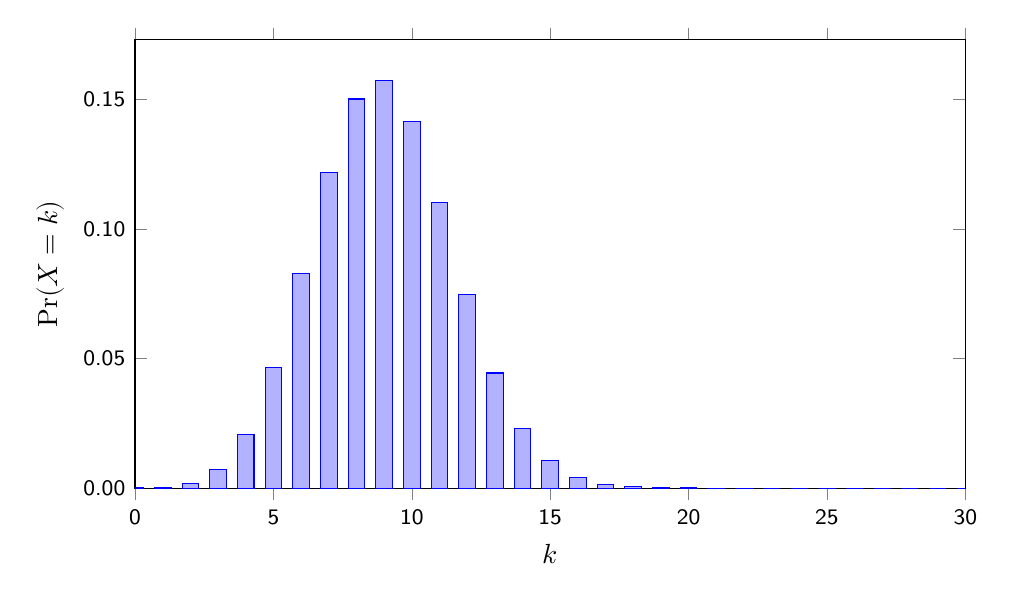
\begin{tikzpicture}[%
declare function={binom(\k,\n,\p)=\n!/(\k!*(\n-\k)!)*\p^\k*(1-\p)^(\n-\k);}]
\pgfmathsetmacro{\binomN}{30}
\begin{axis}[
    width=\textwidth, height=\axisdefaultheight,
    ylabel={$\Pr(X=k)$},
    xlabel={$k$},
    xmin=0, xmax=\binomN,
    ymin=0,
    scaled ticks = false,
    tick label style={/pgf/number format/assume math mode=true, font=\footnotesize\sffamily},
    yticklabel style={/pgf/number format/.cd, fixed, fixed zerofill, precision=2},
        domain=0:\binomN,samples at={0,1,...,\binomN},
    mark options={scale=0.75, blue},
    ybar, bar width = 6pt
        ]
%\addplot[ycomb] {binom(x,\binomN,0.3)};
\addplot {binom(x,\binomN,0.3)};
\end{axis}
\end{tikzpicture}
\end{frame}

\begin{frame}{幾何分布}
\begin{align*}
\Pr(X = k) &= (1-p)^{k-1}p,\quad p=0.3.
\end{align*}
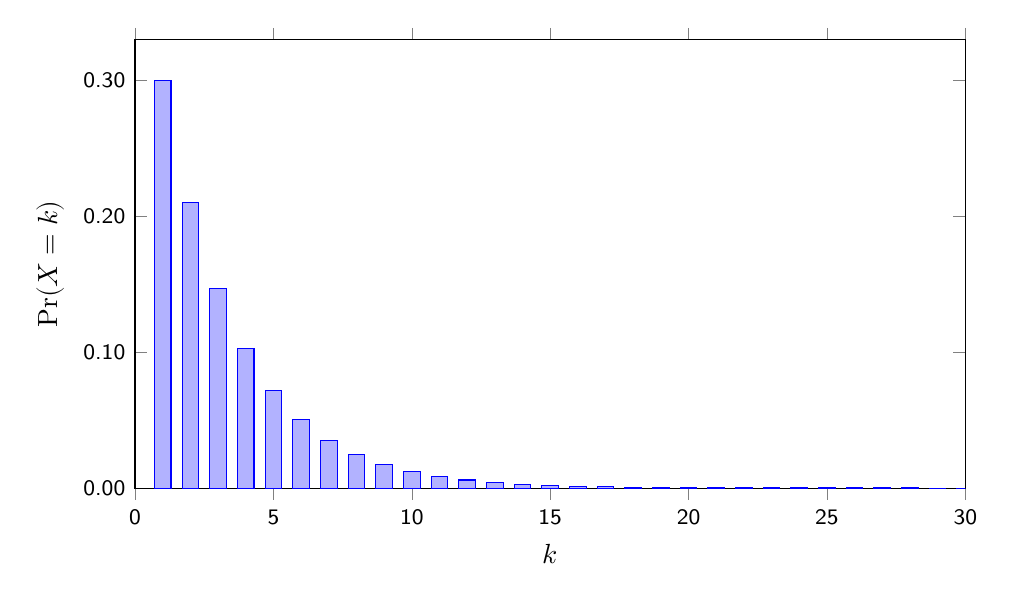
\begin{tikzpicture}[%
declare function={geom(\k,\p)=(1-\p)^(\k-1)*\p;}]
\pgfmathsetmacro{\XMAX}{30}
\begin{axis}[
    width=\textwidth, height=\axisdefaultheight,
    ylabel={$\Pr(X=k)$},
    xlabel={$k$},
    xmin=0, xmax=\XMAX,
    ymin=0,
    scaled ticks = false,
    tick label style={/pgf/number format/assume math mode=true, font=\footnotesize\sffamily},
    yticklabel style={/pgf/number format/.cd, fixed, fixed zerofill, precision=2},
        domain=1:\XMAX,samples at={1,2,...,\XMAX},
    mark options={scale=0.75, blue},
    ybar, bar width = 6pt
        ]
%\addplot[ycomb] {binom(x,\binomN,0.3)};
\addplot {geom(x,0.3)};
\end{axis}
\end{tikzpicture}
\end{frame}

\begin{frame}{負の二項分布}
\begin{align*}
\Pr(X = k) = \binom{r+k-1}{r-1}p^r(1-p)^k,\quad r=5,\, p=0.3.
\end{align*}
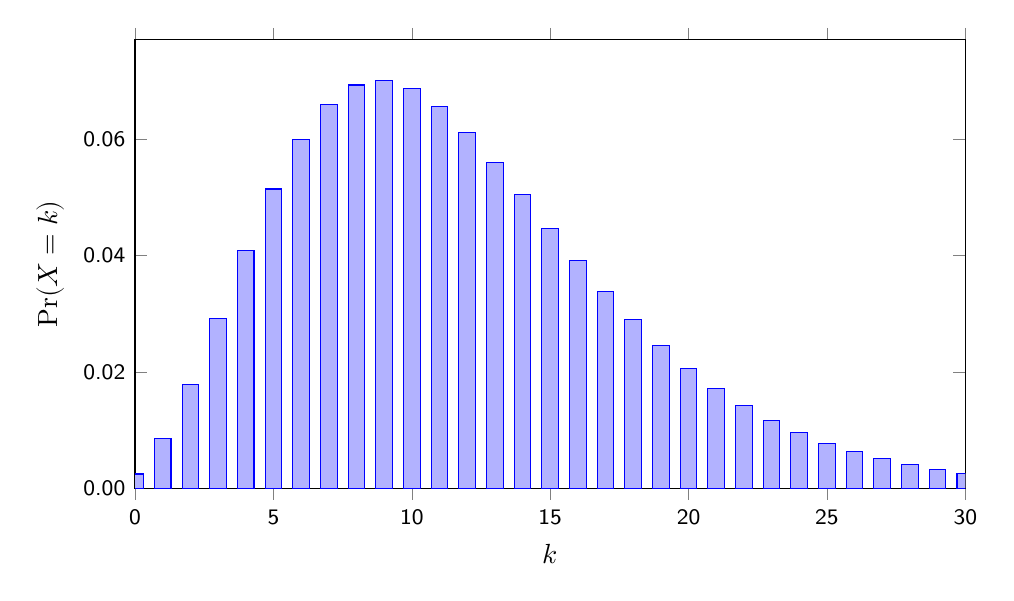
\begin{tikzpicture}[%
declare function={nbinom(\k,\r,\p)=(\r+\k-1)!/(\k!*(\r-1)!)*\p^\r*(1-\p)^\k;}]
\pgfmathsetmacro{\XMAX}{30}
\begin{axis}[
    width=\textwidth, height=\axisdefaultheight,
    ylabel={$\Pr(X=k)$},
    xlabel={$k$},
    xmin=0, xmax=\XMAX,
    ymin=0,
    scaled ticks = false,
    tick label style={/pgf/number format/assume math mode=true, font=\footnotesize\sffamily},
    yticklabel style={/pgf/number format/.cd, fixed, fixed zerofill, precision=2},
        domain=0:\XMAX,samples at={0,1,...,\XMAX},
    mark options={scale=0.75, blue},
    ybar, bar width = 6pt
        ]
%\addplot[ycomb] {binom(x,\binomN,0.3)};
\addplot {nbinom(x,5,0.3)};
\end{axis}
\end{tikzpicture}
\end{frame}

\begin{frame}{超幾何分布}

\vspace{-1em}
\begin{align*}
\Pr(X = k) = \frac{\binom{K}{k}\binom{N-K}{n-k}}{\binom{N}{n}},\quad N=100,\, K=30,\, n=40. 
\end{align*}
%\vfill
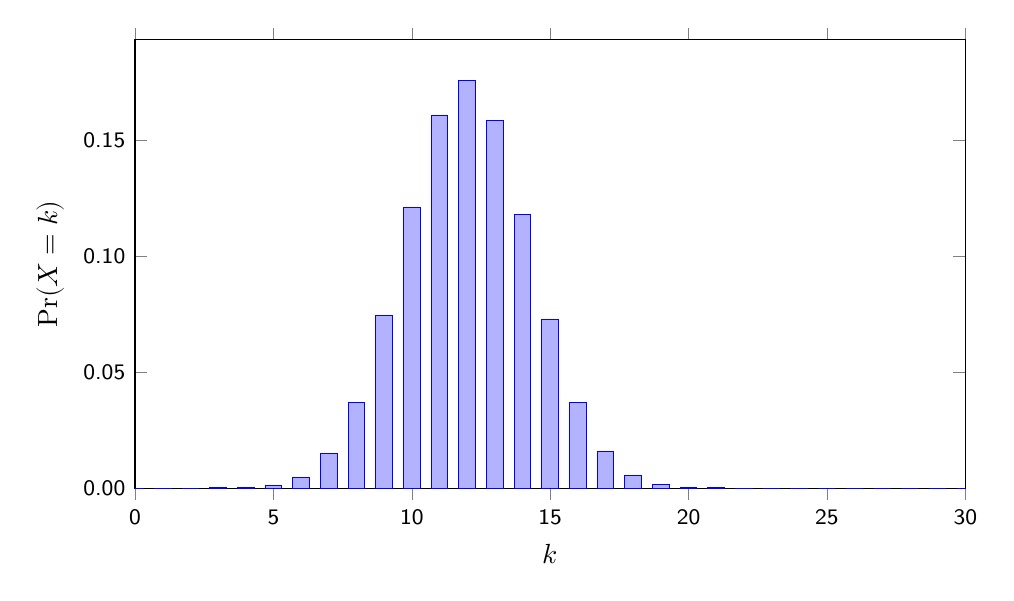
\begin{tikzpicture}[%
declare function={binom(\N,\K)=\N!/(\K!*(\N-\K)!);},
declare function={hypgeom(\k,\N,\K,\n)=binom(\K,\k)*binom(\N-\K,\n-\k)/binom(\N,\n);}]
\pgfmathsetmacro{\XMAX}{30}
\begin{axis}[
    width=\textwidth, height=\axisdefaultheight,
    ylabel={$\Pr(X=k)$},
    xlabel={$k$},
    xmin=0, xmax=\XMAX,
    ymin=0,
    scaled ticks = false,
    tick label style={/pgf/number format/assume math mode=true, font=\footnotesize\sffamily},
    yticklabel style={/pgf/number format/.cd, fixed, fixed zerofill, precision=2},
        domain=0:\XMAX,samples at={0,1,...,\XMAX},
    mark options={scale=0.75, blue},
    ybar, bar width = 6pt
        ]
%\addplot[ycomb] {binom(x,\binomN,0.3)};
\addplot {hypgeom(x,100,\XMAX,40)};
\end{axis}
\end{tikzpicture}
\end{frame}

\begin{frame}{ポアソン分布}
\begin{align*}
\Pr(X = k) &= \frac{\lambda^k}{k!} \mathrm{e}^{-\lambda},\quad\lambda=10
\end{align*}
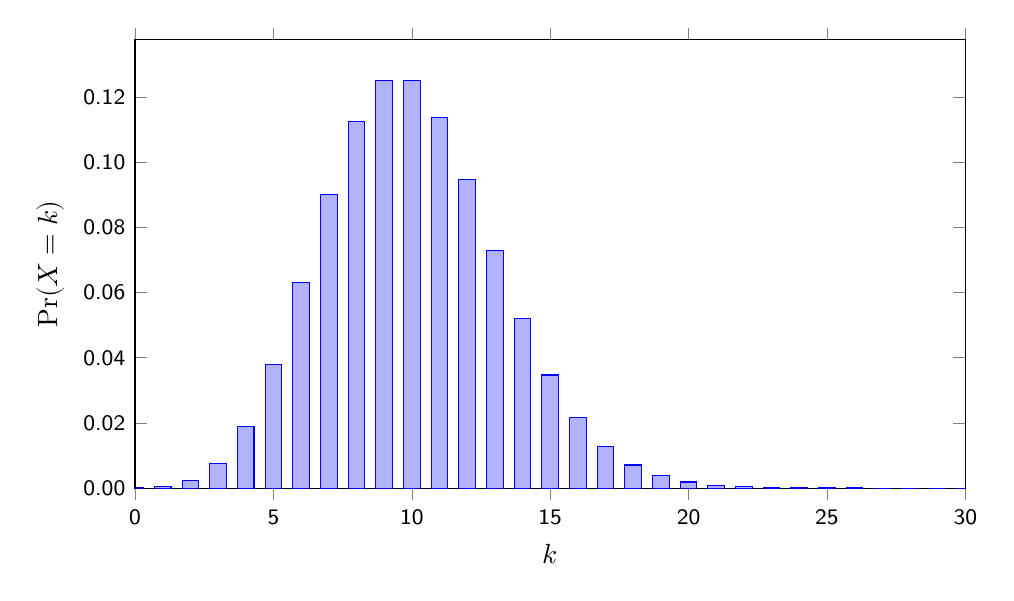
\begin{tikzpicture}[%
declare function={poisson(\k,\l)=\l^\k/\k!*exp(-\l);}]
\pgfmathsetmacro{\XMAX}{30}
\begin{axis}[
    width=\textwidth, height=\axisdefaultheight,
    ylabel={$\Pr(X=k)$},
    xlabel={$k$},
    xmin=0, xmax=\XMAX,
    ymin=0,
    scaled ticks = false,
    tick label style={/pgf/number format/assume math mode=true, font=\footnotesize\sffamily},
    yticklabel style={/pgf/number format/.cd, fixed, fixed zerofill, precision=2},
        domain=0:\XMAX,samples at={0,1,...,\XMAX},
    mark options={scale=0.75, blue},
    ybar, bar width = 6pt
        ]
%\addplot[ycomb] {binom(x,\binomN,0.3)};
\addplot {poisson(x,10)};
\end{axis}
\end{tikzpicture}
\end{frame}


\begin{frame}{同時確率と条件付き確率}
確率変数$X$と$Y$の同時確率
\begin{align*}
\Pr(X=x, Y=y)
\end{align*}
周辺化
\begin{align*}
\Pr(X=x) &= \sum_y \Pr(X=x, Y=y)\\
\Pr(Y=y) &= \sum_x \Pr(X=x, Y=y)
\end{align*}

条件付確率
\begin{align*}
\Pr(X=x\mid Y=y) &= \frac{\Pr(X=x,Y=y)}{\Pr(Y=y)}
\end{align*}
\small $Y=y$のときの$X=x$の確率($\Pr(Y=y)=0$のときは定義されない)
\end{frame}

\begin{frame}{独立確率変数}
確率変数$X$と$Y$が独立$\stackrel{\mathrm{def}}{\iff}\Pr(X=x,Y=y)=\Pr(X=x)\Pr(Y=y)$.

\vspace{2em}
任意の写像$f$と$g$について、

確率変数$X$と$Y$が独立$\implies$ $f(X)$と$g(Y)$は独立。
\end{frame}

\begin{frame}{少数の法則}
\begin{theorem}[少数の法則]
非負実数$\lambda\ge 0$とする。
非負整数$n$について$p_n=\lambda/n$とする。
任意に固定した非負整数$k$について、
\begin{align*}
\lim_{n\to\infty} \binom{n}{k} p_n^k(1-p_n)^{n-k} &= \frac{\lambda^k}{k!}\mathrm{e}^{-\lambda}.
\end{align*}
\end{theorem}
\begin{proof}
\begin{align*}
\lim_{n\to\infty} \binom{n}{k} p_n^k(1-p_n)^{n-k} &= \lim_{n\to\infty} \binom{n}{k} \left(\frac{\lambda}{n}\right)^k\left(1-\frac{\lambda}{n}\right)^{n-k}\\
&= \lim_{n\to\infty} \binom{n}{k} \left(\frac{\lambda}{n}\right)^k\left(1-\frac{\lambda}{n}\right)^{-k}\left(1-\frac{\lambda}{n}\right)^{\frac{n}{\lambda}\lambda}\\
&= \frac{\lambda^k}{k!} \mathrm{e}^{-\lambda}.\qedhere
\end{align*}
\end{proof}
\end{frame}

\end{document}
